\documentclass[../main/main.tex]{subfiles}
\graphicspath{{./figures/}}

\makeatletter
\renewcommand{\@chapapp}{Travaux pratiques -- TP}
\makeatother

% \toggletrue{student}
% \toggletrue{corrige}
% \renewcommand{\mycol}{black}
% \renewcommand{\mycol}{gray}

\hfuzz=5.002pt

\begin{document}
\setcounter{chapter}{22}

\settype{enon}
\settype{solu_prof}
\settype{solu_stud}

\chapter{\cswitch{%
	  Correction du TP
  }{%
	  Titrage du sulfate ferreux par potentiométrie et colorimétrie
  }
 }

\enonce{%
	\begin{tcn}*(exem)<ctc>{\iconhow~Capacités exigibles}
		\begin{itemize}
			\item Identifier et exploiter la réaction support du titrage (recenser les
			      espèces présentes dans le milieu au cours du titrage, repérer
			      l'équivalence, justifier qualitativement l'allure de la courbe ou le
			      changement de couleur observé).
			\item Choisir et utiliser un indicateur coloré de fin de
			      titrage~; distinguer l'équivalence et le virage d'un indicateur
			      coloré de fin de titrage.
		\end{itemize}
	\end{tcn}
	\vspace{-10pt}

	\section{Objectifs}

	\begin{itemize}
		\item Réaliser un titrage potentiométrique à intensité nulle.
		\item Choisir un indicateur coloré redox.
		\item Réaliser un dosage colorimétrique redox.
		\item Vérifier expérimentalement un donnée indiquée par un fabricant.
	\end{itemize}

	\section{S'approprier}
	\subsection{Introduction}
	Le sulfate de fer est utilisé en jardinage pour reverdir et renforcer les
	gazons, bleuir les hortensias et pour éliminer la mousse des pelouses. On peut
	le trouver dans les jardineries sous forme d'une solution aqueuse ayant une
	teneur en fer de $c_{0,m} = \SI{60}{g.L^{-1}}$. Afin de vérifier cette
	concentration, on envisage deux méthodes de titrage d'oxydoréduction.
	\bigbreak
	La solution commerciale de sulfate de fer (solution $S_0$) a été diluée d'un
	facteur $f = 100$ fois pour donner la solution $S_1$ (déjà préparée) de
	concentration $c_1$. Cette dernière est dosée par une solution de sulfate de
	cérium (IV) à la concentration $c_2 = \SI{1.00e-2}{mol.L^{-1}}$
	\begin{tcn}*(defi)<ctc>{\icondata~Données}
		\begin{itemize}
			\item $E_1^\circ(\ce{Fe^{3+}/Fe^{2+}}) = \SI{0.68}{V}$
			\item $M (\ce{Fe}) = \SI{55.8}{g.mol^{-1}}$
			\item $E_2^\circ (\ce{Ce^{4+}/Ce^{3+}}) = \SI{1.44}{V}$
			\item $M (\ce{Ce}) = \SI{140.1}{g.mol^{-1}}$
		\end{itemize}
	\end{tcn}

	\subsection{Titrage potentiométrique à intensité nulle}
	\subsubsection{Principe général}
	Un titrage potentiométrique consiste à mesurer la différence de potentiel entre
	une électrode de mesure et une électrode de référence plongées dans la solution
	à étudier. Cette différence de potentiel est mesurée par un millivoltmètre
	électronique à haute impédance (pour que le courant traversant l'ensemble puisse
	être supposé nul).

	\subsubsection{Électrodes utilisées}
	L'électrode de mesure est, suivant la nature des couples mis en jeu, soit une
	électrode inattaquable quand les espèces redox sont toutes en solution, soit une
	électrode métallique constituant la forme réduite de l'un des couples présents
	en solution. Ici toutes les espèces redox sont en solution, on utilise alors une
	électrode de platine.
	\bigbreak
	Une électrode de référence est une électrode dont le potentiel peut être
	considéré comme constant, à une température donnée, quelle que soit la solution
	avec laquelle elle est mise en contact. L'électrode de référence utilisée le
	plus couramment dans le passé était l'électrode au calomel saturée (E.C.S.).
	Mais cette électrode contenait du mercure, métal dangereux pour l'homme comme
	pour l'environnement. Elles sont maintenant le plus souvent remplacée par une
	électrode argent/chlorure d'argent. Le
	\bigbreak
	Le potentiel de cette électrode par rapport à l'E.S.H. est $E\ind{ref} =
		\SI{197}{mV}$ à \SI{25}{\degreeCelsius}. Ainsi, en notant $U$ la tension lue au
	millivoltmètre haute impédance entre l'électrode de mesure et l'électrode de
	référence, et $E$ le potentiel de la solution lue par l'électrode de mesure, on
	a
	\[
		U = E - E\ind{ref}
		\Lra
		\boxed{E = U + E\ind{ref}}
	\]

	\subsection{Titrage colorimétrique redox}
	Ces titrages utilisent un indicateur redox de fin de réaction afin de repérer
	l'équivalence. Un indicateur coloré d'oxydoréduction est une espèce chimique
	(souvent organique) dont les formes oxydée et réduite ont des couleurs
	différentes. Il est caractérisé par son potentiel standard.
}%

\setcounter{section}{2}
\section{Analyser}
\subsection{Réaction de dosage}
\setlist[blocQR,1]{leftmargin=10pt, label=\clenumi}
\QR{%
	Écrire la réaction de titrage des ions \ce{Fe^{2+}} par les ions \ce{Ce^{4+}}.
}{%
	\leavevmode\vspace*{-15pt}\relax
	\[
		\ce{Fe^{2+}_{\aqu} + Ce^{4+}_{\aqu} = Fe^{3+}_{\aqu} + Ce^{3+}_{\aqu}}
	\]
}%
\QR{%
	Montrer, à l'aide d'un diagramme de prédominance, que sa constante s'écrit
	\[
		K^\circ = 10^{\DS \frac{E_2^\circ-E_1^\circ}{\num{0.06}}}
	\]
	La calculer et discuter de la faisabilité d'un titrage avec une telle
	réaction. Quelle information manque-t-il pour conclure~?
}{%
	\noindent
	\begin{minipage}[t]{.650\linewidth}
		Avec un électron échangé, on voit que la réaction est favorisée donc on prend
		bien la valeur absolue de la différence des $E^\circ$. On obtient
		\[
			\xul{K^\circ = 10^{\num{12.7}}}
		\]
	\end{minipage}
	\hfill
	\begin{minipage}[t]{.35\linewidth}
		\vspace{0pt}
		\begin{center}
			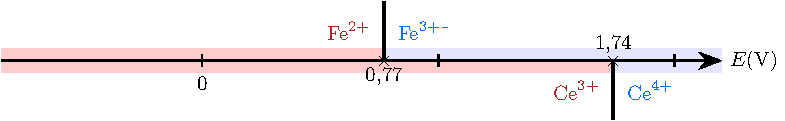
\includegraphics[width=\linewidth]{predom_2}
		\end{center}
	\end{minipage}
	et elle est donc bien totale, ce qui est nécessaire pour être un support de
	titrage~; on ne sait par contre rien sur la cinétique, or il faut qu'elle soit
	également rapide, ce qui n'est pas indiqué.
}%
\QR{%
	Compte-tenu des informations fournies par le fabricant, estimer le volume
	équivalent attendu lors du titrage de $V_1 = \SI{10.00}{mL}$ de la solution
	$S_1$ par la solution de sulfate de cérium (IV).
}{%
	\leavevmode\vspace*{-15pt}\relax
	\begin{gather*}
		\beforetext{Compte-tenu de la stœchiométrie,}
		\boxed{c_1V_1 = c_2V\ind{2,eqv}}
		\\
		\beforetext{Or,}
		c_1 = \frac{c_{0,m}}{fM}
		\qdc
		\boxed{V\ind{2,eqv} = \frac{c_{0,m}V_1}{fMc_2}}
		\qav
		\left\{
		\begin{array}{rcl}
			c_{0,m}     & = & \SI{60}{g.L^{-1}}
			\\
			M (\ce{Fe}) & = & \SI{55.8}{g.mol^{-1}}
			\\
			V_1         & = & \SI{10.00e-3}{L}
			\\
			c_2         & = & \SI{1.00e-2}{mol.L^{-1}}
			\\
			f           & = & 100
		\end{array}
		\right.\\
		\AN
		\xul{
			V\ind{2,eqv} = \SI{10.8}{mL}
		}
	\end{gather*}
}%

\subsection{Titrage colorimétrique par oxydoréduction}
\enonce{%
	L'équivalence peut être repérée en utilisant un indicateur coloré
	d'oxydoréduction introduit en faible quantité (pour que sa réaction parasite ne
	modifie pas de manière sensible la position de l'équilibre). Il s'agit d'une
	substance intervenant dans un couple oxydant-réducteur
	$\ce{Ox\ind{ind}/Red\ind{ind}}$ dont les formes oxydée et réduite n'ont pas la
	même couleur (les deux formes sont dissoutes). Le changement de couleur de
	l'indicateur a lieu autour du potentiel $E =
		E^\circ(\ce{Ox\ind{ind}/Red\ind{ind}})$. Un indicateur convenable aura son
	changement de couleur lors de l'équivalence~; ainsi, si on note $E\ind{eqv}$ le
	potentiel atteint au moment de l'équivalence, un indicateur adapté vérifiera
	$\boxed{E^\circ(\ce{Ox\ind{ind}/Red\ind{ind}}) \approx E\ind{eqv}}$.
}%
\QR{%
	\leftcenters{%
		Montrer qu'on a ici
	}{%
		$E\ind{eqv} = \frac{1}{2}(E_2^\circ + E_1^\circ)$
	}%
}{%
	\leavevmode\vspace*{-15pt}\relax
	\begin{center}
		\def\rhgt{0.35}
		\centering
		\begin{tabularx}{\linewidth}{|l|c||YdYdYdY|}
			\hline
			\multicolumn{2}{|c||}{
				$\xmathstrut{\rhgt}$
			\textbf{Équation}}    &
			$\ce{Fe^{2+}_{\aqu}}$ & $+$                  &
			$\ce{Ce^{4+}_{\aqu}}$ & $\ra$                &
			$\ce{Fe^{3+}_{\aqu}}$ & $+$                  &
			$\ce{Ce^{3+}_{\aqu}}$                          \\
			\hline
			$\xmathstrut{\rhgt}$
			Initial               & $\xi = 0$            &
			$c_1V_1$              & \vline               &
			$c_2V\ind{2,eqv}$     & \vline               &
			$0$                   & \vline               &
			$0$                                            \\
			\hline
			$\xmathstrut{\rhgt}$
			Final                 & $\xi_f = \xi_{\equ}$ &
			$\ep$                 & \vline               &
			$\ep$                 & \vline               &
			$\xi_{\equ}$          & \vline               &
			$\xi_{\equ}$                                   \\
			\hline
		\end{tabularx}
	\end{center}
	\leavevmode\vspace*{-15pt}\relax
	\begin{gather*}
		\beforetext{Par unicité du potentiel, on a}
		E\ind{eqv} = E_1 = E_2
		\\\beforetext{Or}
		K^\circ = \frac{\xi\ind{eq}^2}{\ep^2} = 10^{\DS
				\frac{E_2^\circ-E_1^\circ}{\num{0.06}}}
		\qet
		E_1 = E_1^\circ + \num{0.06} \log \frac{\xi\ind{eq}}{\ep}
		\\\beforetext{Soit}
		E\ind{eq} =
		E_1^\circ + \frac{\num{0.06}}{2} \log 10^{\DS
				\frac{E_2^\circ-E_1^\circ}{\num{0.06}}} =
		E_1^\circ + \frac{E_2^\circ-E_1^\circ}{2}
		\\\beforetext{Ainsi}
		\boxed{E\ind{eq} = \frac{E_1^\circ+E_2^\circ}{2}}
		\qed
	\end{gather*}
}%

\section{Réaliser et valider}
\subsection{Dosage potentiométrique}
\subsubsection{Protocole}
\enonce{%
	\begin{tcb}*(expe)<itc>"chem"{Dosage potentiométrique}
		\begin{enumerate}
			\item Prélever $V_1 = \SI{10.00}{mL}$ de la solution $S_1$ et les placer
			      dans un bécher.
			\item Rajouter de l'eau en excès pour que les électrodes plongent
			      convenablement. Plonger donc les électrodes.
			\item Réaliser le titrage et relever la valeur de $U = \Delta{E}$ tous les
			      \SI{1}{mL} d'abord~; \textbf{vous resserrerez les mesures autour de
				      l'équivalence}.
			\item Tracer la courbe $U =f(V)$ sur le logiciel de votre choix.
		\end{enumerate}
	\end{tcb}
}%

\setlist[blocQR,1]{leftmargin=10pt, label=\sqenumi}
\QR{%
	Faire un schéma du protocole expérimental.
}{%
	Non corrigé.
}%
\QR{%
	Préciser le rôle de chaque électrode.
}{%
	solu
}%

\subsubsection{Exploitation des résultats}
\QR{%
	Le passage par l'équivalence est caractérisé par un saut de potentiel. En
	déduire une méthode de repérage de l'équivalence, qui ne soit \textbf{pas} la
	méthode des tangente. La mettre alors en œuvre pour déterminer le volume
	équivalent.
}{%
	On peut effectuer une \textbf{dérivée numérique} pour repérer le saut. Pour
	les résultats, voir \texttt{Capytale}
	\url{https://capytale2.ac-paris.fr/web/c/2da2-3377150}.
}%
\QR{%
	En déduire la concentration $c_{0,m}$, et calculer son écart relatif avec la
	valeur annoncée.
}{%
	\leavevmode\vspace*{-15pt}\relax
	\begin{gather*}
		\boxed{c_{0,m} = c_2\frac{V\ind{2,eqv}}{V_1}\times f M}
		\qav
		\left\{
		\begin{array}{rcl}
			c_2          & = & \SI{1.00e-2}{mol.L^{-1}}
			\\
			V_1          & = & \SI{10.00}{mL}
			\\
			V\ind{2,eqv} & = & \SI{10.00}{mL}
			\\
			M (\ce{Fe})  & = & \SI{55.8}{g.mol^{-1}}
			\\
			f            & = & 100
		\end{array}
		\right.\\
		\AN
		\xul{
			c_{0,m} = \SI{56}{g.L^{-1}}
		}
		\Ra
		\xul{\ep_r = \num{0.91}}
	\end{gather*}
}%

\subsection{Titrage colorimétrique}
\subsubsection{Choix de l'indicateur}
\QR{%
	Parmi les indicateurs suivants, lequel est le plus adapté au titrage~?
	\begin{center}
		\begin{tabular}{lccc}
			\toprule
			\textbf{Indicateur}        &
			\textbf{Couleur oxydant}   &
			\textbf{Couleur réducteur} &
			$E^\circ~(\si{mV})$
			\\
			Bleu de méthylène          &
			Bleu                       &
			Incolore                   &
			\num{520}
			\\
			Diphénylamine              &
			Violet                     & Incolore & \num{760}
			\\
			Orthophénantroline         &
			Bleu pâle                  & Rouge    & \num{1060}
			\\
			\bottomrule
		\end{tabular}
	\end{center}
}{%
	C'est le…
}%

\subsubsection{Protocole et exploitation}
\enonce{%
	\begin{tcb}*(expe)<itc>"chem"{Titrage colorimétrique}
		Réaliser le titrage.
	\end{tcb}
}%
\QR{%
	En déduire la concentration $c_{0,m}$, et calculer son écart relatif avec la
	valeur annoncée.
}{%
	solu
}%

\subsection{Propagation des incertitudes}
\enonce{%
	On veut déterminer l'incertitude-type sur $c_0$, notée $u(c_0)$. Pour cela, il
	nous faut les incertitudes de toutes les valeurs dont elle dépend.
}%
\QR{%
	Mettez en commun vos valeurs de $V\ind{2,eqv}$ pour en déduire les valeurs
	mesurées avec incertitude \textbf{pour chaque dosage}~: vous ferez donc
	attention à bien nommer vos variables (suggestion~: \texttt{V2eq\_col} et
	\texttt{V2eq\_pot}). Utilisez pour cela le lien suivant~:
	\url{https://capytale2.ac-paris.fr/web/c/cd2f-3377099}
}{%
	Voir \url{https://capytale2.ac-paris.fr/web/c/2da2-3377150}
}%
\QR{%
	On suppose $u(c_2)/c_2 = 1\%$ et $u(f)/f = 1\%$, avec $f$ le facteur de
	dilution. Justifier les valeurs des autres incertitudes, puis appliquer alors
	la méthode \textsc{Monte-Carlo} et écrivez le résultat sous la forme $c_0 \pm
		u(c_0)$
}{%
	Idem.
}%

\section{Conclure}
\QR{%
	Parmi les deux méthodes proposées, laquelle vous semble la plus précise~? la
	plus rapide~? Les indications fournies par le vendeur du produit sont-elles
	fiables~?
}{%
	solu
}%

\end{document}
